\subsection{Analysis of Toy Data}\label{Toy Data}

\textbf{Property}. If every DC has $\infty$ slots, then Greedy Approach yields the optimal solution.

As the amount of slots is infinity, assign one task will never worsen the data transferring time of others tasks. Thus, we can assign each task to its optimal position and this results an optimal solution of all jobs. The property enables us to find the optimal solution of toy data. 

In fact, DCs in toy data have relatively large slots amount. Applying Greedy Approach on toy data exactly yields the optimal solution. Beside, Network-Flow-Based Greedy Approach and Network-Flow-Based Fair Approach also yields this optimal solution while K-Greedy may sometimes yields a better time.

\begin{figure}[htb]
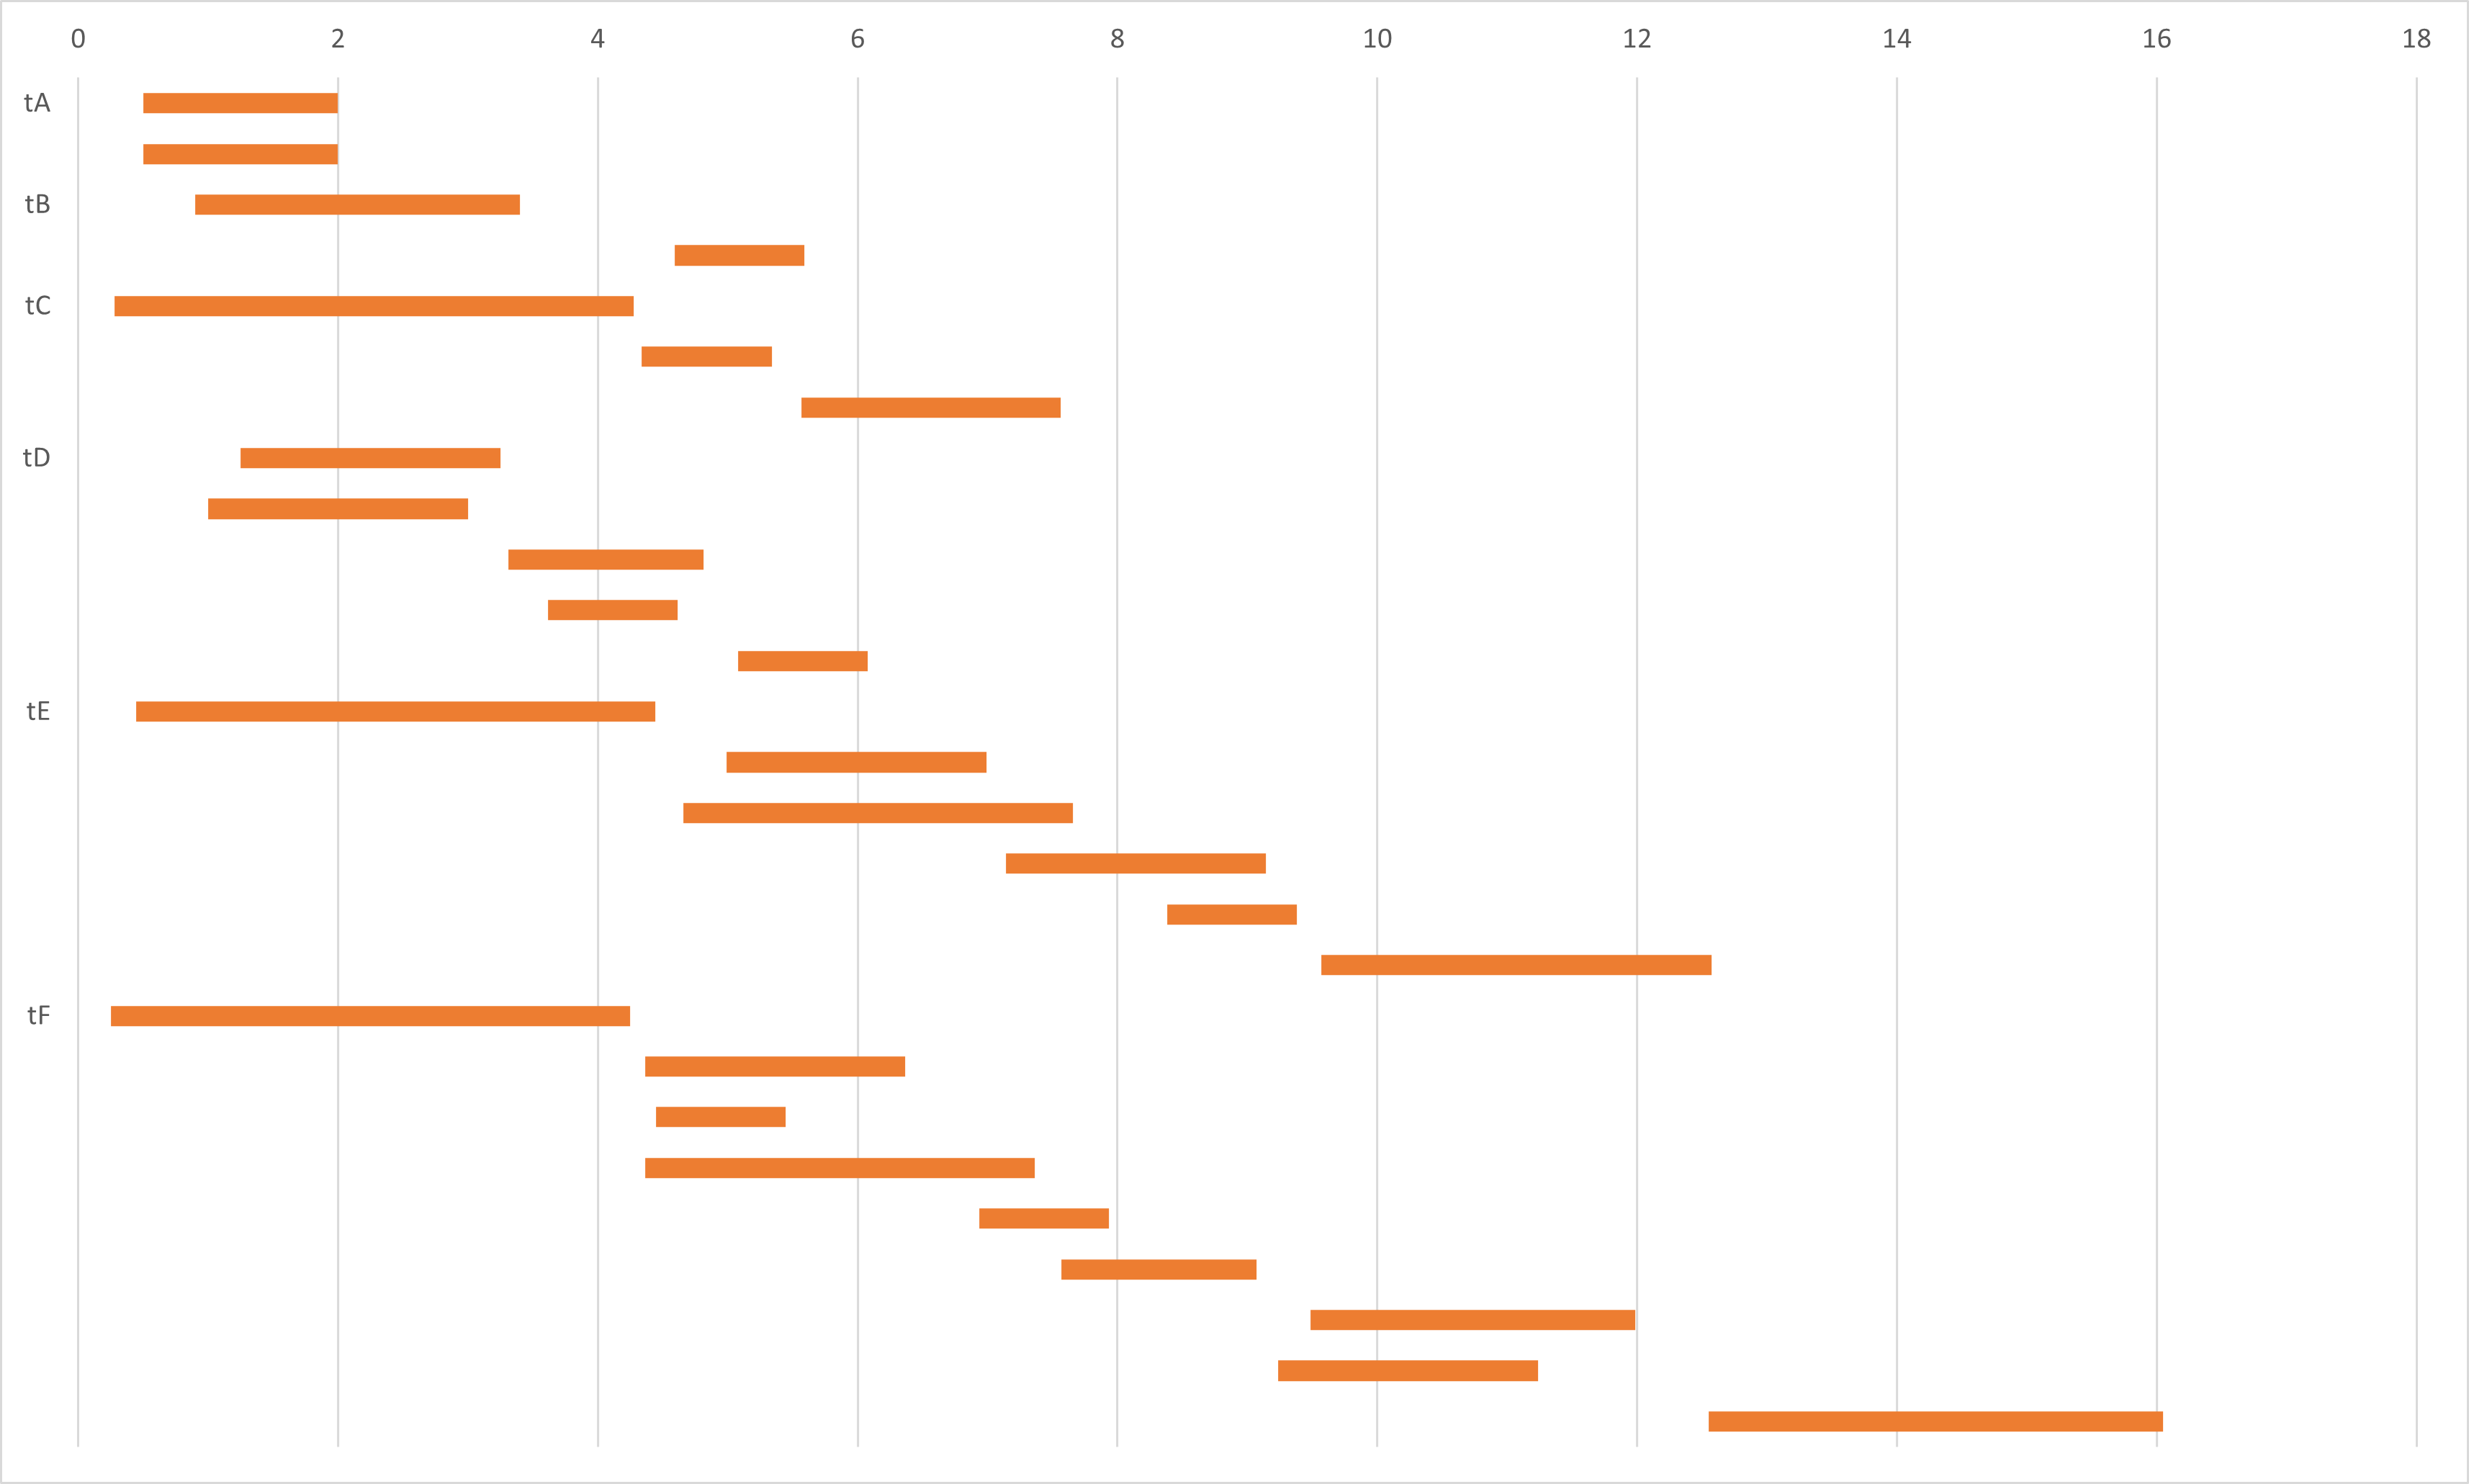
\includegraphics[width=0.8\textwidth]{figure/fig-toy.png}
\centering
\caption{Gantt chart of the optimal solution} \label{fig-toy}
\end{figure}

The solution is better illustrated by Fig. \ref{fig-toy}. The figure shows the start and finish time of each task.
